\documentclass[12pt, titlepage]{article}

\usepackage{booktabs}
\usepackage{tabularx}
\usepackage{hyperref}
\usepackage{graphicx}
\hypersetup{
    colorlinks,
    citecolor=black,
    filecolor=black,
    linkcolor=red,
    urlcolor=blue
}
\usepackage[round]{natbib}
\usepackage{enumerate}
\usepackage{float}

\title{SE 3XA3: Software Requirements Specification\\Namcap}

\author{Team 2, VPB Game Studio
		\\ Prajvin Jalan (jalanp)
		\\ Vatsal Shukla (shuklv2)
		\\ Baltej Toor (toorbs)
}

\date{\today}

%% Comments

\usepackage{color}

\newif\ifcomments\commentstrue

\ifcomments
\newcommand{\authornote}[3]{\textcolor{#1}{[#3 ---#2]}}
\newcommand{\todo}[1]{\textcolor{red}{[TODO: #1]}}
\else
\newcommand{\authornote}[3]{}
\newcommand{\todo}[1]{}
\fi

\newcommand{\wss}[1]{\authornote{blue}{SS}{#1}}
\newcommand{\ds}[1]{\authornote{red}{DS}{#1}}
\newcommand{\mj}[1]{\authornote{red}{MSN}{#1}}
\newcommand{\cm}[1]{\authornote{red}{CM}{#1}}
\newcommand{\mh}[1]{\authornote{red}{MH}{#1}}

% team members should be added for each team, like the following
% all comments left by the TAs or the instructor should be addressed
% by a corresponding comment from the Team

\newcommand{\tm}[1]{\authornote{magenta}{Team}{#1}}


\begin{document}

\maketitle

\pagenumbering{roman}
\tableofcontents
\listoftables
\listoffigures

\newpage

\begin{table}[H]
\caption{\bf Revision History}
\begin{tabularx}{\textwidth}{p{3cm}p{2cm}X}
\toprule {\bf Date} & {\bf Version} & {\bf Notes}\\
\midrule
2016-10-11 & 1.0 & Addition of content to Project Drivers sections excluding Naming Conventions and Terminology\\
2016-10-11 & 1.1 & Addition of content to Project Issues sections excluding Open Issues and Ideas for Solutions\\
2016-10-11 & 1.2 & Addition of content to Non-functional Requirements section\\
2016-10-11 & 1.3 & Formatting fixes to figure and table locations\\
2016-10-11 & 1.4 & Further formatting and content additions to 1.4 and 4.10\\
2016-10-11 & 1.5 & Revision of linguistics and use of 'Pacman' in the document\\
2016-10-11 & 1.6 & Addition of Symbolic Paremeters table and minor text edits\\
2016-10-29 & 1.7 & Revision of Mandated Constraints section to reference feedback\\
2016-10-30 & 1.8 & Revision of Legal Requirements section to reference feedback\\
2016-10-31 & 1.9 & Revision of Functional Requirements to address Big Dot functionality feedback\\
\bottomrule
\end{tabularx}
\end{table}

\newpage

\pagenumbering{arabic}

This document describes the requirements for the redevelopment project Namcap.  The template for the Software
Requirements Specification (SRS) is a subset of the Volere
template~\citep{RobertsonAndRobertson2012}.

\section{Project Drivers}

\subsection{The Purpose of the Project}
\paragraph{}
The purpose of this project is to redevelop the classic arcade game Pacman based on an unstructured open-source development. The Pacman conceptual redevelopment, '‘Namcap' aims to provide the classic arcade-style experience to a broader player base. The project will be geared towards a computer implementation to provide the most access for the classical gaming interaction without having to pay large amounts for additional hardware. The project will focus on redeveloping the reference open-source project with correct programming standards, modularization, and an emphasis on formal documentation.

\subsection{The Stakeholders}

\subsubsection{The Client}
\paragraph{}
The project is being developed for an external entity that has final say on the acceptance of the redevelopment and will review the project before deployment. The external entity shows interest in the redevelopment of open source projects with emphasis on improvement of programming structure and documentation.

\subsubsection{The Customers}
\paragraph{}
The general gaming population are customers for this project. A typical gamer would have access to the internet and have the computer experience to download and run the application. 

\subsubsection{Other Stakeholders}
\paragraph{}
Another stakeholder of this project is the redevelopment team. VPB Game Studio is responsible for the development of Namcap, with emphasis on the utilization of correct programming principles and formalization of documentation throughout development.

\subsection{Mandated Constraints}

\subsubsection{Solution Constraints}
\paragraph{}
The implementation shall be based on the same mechanics as the original implementation. Mechanics such as sprit movement, collision with various in-game entities, and scoring should reflect Pacman. The project is a redevelopment and aims to stay true to the retro-arcade gaming interaction that Pacman utilized. 

\subsubsection{Implementation Environment of the Current System}
\begin{enumerate}[i]
\item All controls associated with the game mechanics shall be integrated to work with any keyboard configuration.
\item The application shall be executable on both Mac, Windows, and Linux operating systems.
\end{enumerate} 

\subsubsection{Partner or Collaborative Applications}
\paragraph{}
%\textcolor{red}{Consider any libraries or development kits that could fall in this category - CM} \\
%The section now specifies the JDK and built-in libraries as possible partner/collaborative applications.
The implementation requires the Java Development Kit along with several built-in libraries. The libraries to be utilized will cover various aspects of the implementation from GUI to testing elements.

\subsubsection{Off-the-Shelf Software}
\paragraph{}
The implementation is self-contained and therefore requires no addition OTS software to be incorporated into the project.

\subsubsection{Anticipated Workplace Environment}
\paragraph{}
The application shall be usable on desktop and laptop computer platforms. This allows users, once the application is downloaded locally, to run the game virtually anywhere with a laptop. The implementation does not affect the workplace environment externally as no audio functionality is built-in. The execution of the implementation is only limited to the extent of laptop portability.
 
\subsubsection{Schedule Constraints}
\paragraph{}
%\textcolor{red}{ The self imposed deadlines are perfectly applicable as valid schedule constraints - CM} \\
%Provided reference to the Gantt Project for detailed description of the project scheduling constraints.
Self-imposed scheduling deadlines have been put in place for the development process. Specifically, the development team is aiming to have the initial implementation fully functioning by December 2016. For a more specific break-down of the established development deadlines, refer to the Namcap Gantt Project.

\subsubsection{Budget Constraints}
\paragraph{}
%\textcolor{red}{In this case, I would consider using "Man-Hours" as a budget of which is constrained by other projects / school - CM} \\
%Reference to man-hours as a budgetary constraint.
In terms of this redevelopment project, man-hours is the primary budgetary constraint. The time of the developers is split between this redevelopment and other projects/ courses varying for each individual. This results in a man-hour constraint of 10 hours/week to account for the individual schedules of the development team.  Since the redevelopment is based on an open-source implementation, any and all additional resources for the project are readily and freely available.

\subsubsection{Enterprise Constraints}
\paragraph{}
The redeveloped implementation shall follow the correct programming and development standards as well as emphasis the creation of formalized documentation.

\subsection{Naming Conventions and Terminology}
\begin{table}[H]
\caption{Terminology} \label{tab:terms}
\begin{center}
\begin{tabular}{| c | l |}
\hline
\textbf{Terminology Used} & \textbf{Meaning/Reference To} \\ \hline
OTS & 'Off-The-Shelf' solution \\ \hline
UI & 'User Interface' \\ \hline
AI & 'Artificial Intelligence' \\ \hline
NF/F & 'Non-Functional/Functional' \\ \hline
Project/Redevelopment & Recreation of Pacman, Namcap \\ \hline
Player & In-game player entity (character icon)\\
\hline
\end{tabular}
\end{center}
\end{table}

\subsection{Relevant Facts and Assumptions}

\subsubsection{Relevant Facts}
\begin{enumerate}[i]
\item The existing base implementation is approximately 1600 lines of Java code.
\item The original project is to be used as a source to conceptualize based on the requirements. No code will be used from the original project.
\end{enumerate}

\subsubsection{Business Rules}
\paragraph{}
The redevelopment team shall delegate work as to equalize the amount taken on by each member. This allows for an efficient development process and is mandated by the client of the project.

\subsubsection{Assumptions}
\paragraph{}
The redevelopment project assumes that:
\begin{enumerate}[i]
\item All required software components (IDEs, Image Editing Software) will be readily available.
\item Audio functionality shall not be implemented initially (may be implemented in the future following the appropriate decision process).
\item The implementation will be executed in a verified instance of either the Mac, Windows, or Linux operating systems.
\item The majority of users will have basic computer knowledge and experience.
\end{enumerate}

\section{Functional Requirements}

\subsection{The Scope of the Work and the Product}

\subsubsection{The Context of the Work}
The context diagram of the work is given in \hyperref[fig:gamecontext]{Figure~\ref*{fig:gamecontext}}.
\begin{figure}[H]
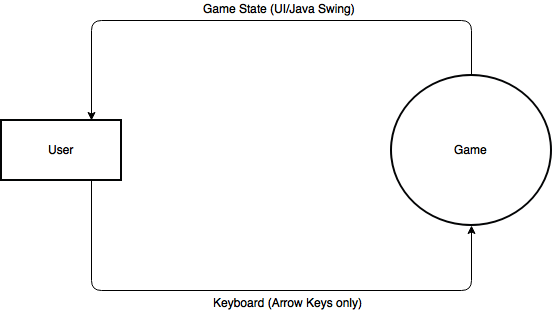
\includegraphics[width=\textwidth]{gamecontext}
\caption{Context Diagram of the Work} \label{fig:gamecontext}
\end{figure}

\subsubsection{Work Partitioning}
\hyperref[fig:flow-3]{Figure~\ref*{fig:flow-3}} demonstrates a rough representation of the mechanics of the game. The user interface contains a main menu, a game over screen and the in-game interface where all of the gameplay will occur.

\begin{figure}[H]
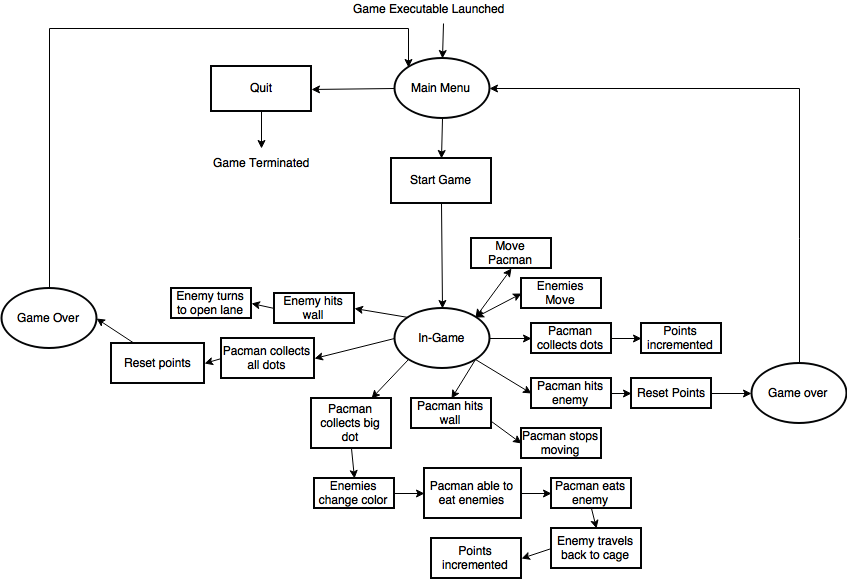
\includegraphics[width=\textwidth]{flow-3}
\caption{Flow Diagram of the Game} \label{fig:flow-3}
\end{figure}

\subsubsection{Individual Product Use Cases}

\begin{table}[H]
\caption{List of events} \label{tab:events}
\begin{tabularx}{\textwidth}{| p{3cm} | p{4cm} | X |}
\toprule {\bf Event Name} & {\bf Inputs/Outputs} & {\bf Summary}\\
\midrule
Start Game & Keyboard (Spacebar) & The game is started.\\ \hline
Move Player & Keyboard(arrow keys)/UI(ouput) & Player moves through the map.\\ \hline
Enemies Move & UI(output) & The enemies move through the map.\\ \hline
Player hits wall & Keyboard(arrow keys)/UI(output) & Player stops moving unless a valid move is made.\\ \hline
Player collects dots & Keyboard(arrow keys)/UI(output) & Player collects dots which increases the game points.\\ \hline
Player hits enemy & Keyboard(arrow keys)/UI(output) & Points are reset and UI changes to main menu if player lives == 0. Lives decrement by 1 otherwise.\\ \hline
Player collects big dot & Keyboard(arrow keys)/UI(output) & Player collects big dot, enemies change colour and Player is able to hit the enemies. Points are incremented as Player hits enemies.\\ \hline
Player collects all dots & Keyboard(arrow keys)/UI(output) & Once Player collects all dots, the points are reset and UI switches back to main menu.\\ \hline
Enemy hits wall & UI(output) & When enemies hit a wall, they will turn and start moving to a valid path.\\ \hline
Player collides with Enemy (with Big Dot consumed/active) & Keyboard(arrow keys)/UI(output) & Player collides with enemies with Big Dot consumed and points are incremented by double standard point value. Enemy is removed by collision and respawns in the center of the level.\\
\bottomrule
\end{tabularx}
\end{table}
%\textcolor{red}{ Include Player colliding with Enemy when Big Dot is consumed - CM} \\
%Big Dot active collision functionality has been addressed and the appropriate requirements have been added
\begin{itemize}
\item
Use Case Number: 1

Name: Start Game

Trigger: The user starts a new game.

Precondition: The main menu is open.

Postcondition: The in-game UI is shown and the game is started.

\end{itemize}

\begin{itemize}
\item
Use Case Number: 2

Name: Move Player

Trigger: User presses arrow keys from the keyboard.

Precondition: In-game UI is active.

Postcondition: Player moves according to the arrow pressed.
\end{itemize}

\begin{itemize}
\item
Use Case Number: 3

Name: Player contacts wall

Trigger: Player moves towards a wall.

Precondition: In-game UI is active.

Postcondition: User presses an arrow key to move Player away from wall.

\end{itemize}

\begin{itemize}
\item
Use Case Number: 4

Name: Player contacts enemy

Trigger: Player and enemy collide.

Precondition: In-game UI is active.

Postcondition: Points are reset and main menu UI is active if player lives == 0. Decrements lives by 1 otherwise.
\end{itemize}

\begin{itemize}
\item
Use Case Number: 5

Name: Enemies move

Trigger: Enemies collide with wall.

Precondition: In-game UI is active.

Postcondition: Enemies move according to their AI.
\end{itemize}

\begin{itemize}
\item
Use Case Number: 6

Name: Player collects dots

Trigger: User moves Player towards dots.

Precondition: Dots exist and in-game UI is active.

Postcondition: Points are incremented and the collected dot is no longer visible.
\end{itemize}

\begin{itemize}
\item
Use Case Number: 7

Name: Player collects big dot

Trigger: User moves Player towards big dot.

Precondition: Big dot exists and in-game UI is active.

Postcondition: Enemies change colour and Player is able to collide with enemies.
\end{itemize}

\begin{itemize}
\item
Use Case Number: 8

Name: Player collects last dot

Trigger: User moves Player towards last dot.

Precondition: In-game UI is active.

Postcondition: Points are rest and game over UI is active.
\end{itemize}

\begin{itemize}
\item
Use Case Number: 9

Name: Quit game

Trigger: User presses Escape on the keyboard.

Precondition: Main menu UI is active.

Postcondition: The game application is terminated.
\end{itemize}

\begin{itemize}
\item
Use Case Number: 10

Name: Player collides with Enemy (while Big Dot consumed)

Trigger: User moves player towards enemy with Big Dot active.

Precondition: In-game UI is active. Big Dot is active (indicated by different enemy colour).

Postcondition: Points are incremented by double standard value per each enemy collision. Enemy is removed after collision and respawns at the center of the level.
\end{itemize}


\subsection{Functional Requirements}

\begin{itemize}
\item
Requirement Number: F1

Requirement Type: 2.2

Use Case: 1

Description: User must have the ability to start a new game.

Rationale: The user needs to have this ability in order to play the game.

Fit Criterion: The game is able to be started.

Priority: High

Conflicts: None
\end{itemize}

\begin{itemize}
\item
Requirement Number: F2

Requirement Type: 2.2

Use Case: 2

Description: The user must have the ability to move Player up, down, left or right.

Rationale: The user must have this ability to collect points and dodge enemies.

Fit Criterion: Player moves correctly based on the user’s input.

Priority: High

Conflicts: None
\end{itemize}

\begin{itemize}
\item
Requirement Number: F3 

Requirement Type: 2.2

Use Case: 3

Description: Player must stop moving when coming in contact with a wall.

Rationale: Player must stop when touching a wall to make the game more challenging and fair.

Fit Criterion: Player is unable to pass through walls.

Priority: High

Conflicts: None
\end{itemize}

\begin{itemize}
\item
Requirement Number: F4

Requirement Type: 2.2

Use Case: 4

Description: The game must come to an end when Player comes in contact with an enemy.

Rationale: Player must ''die'' when coming in contact with an enemy to make the game more challenging and fair.

Fit Criterion: Player is unable to pass through enemies.

Priority: High

Conflicts: None
\end{itemize}

\begin{itemize}
\item
Requirement Number: F5

Requirement Type: 2.2

Use Case: 5

Description: The enemies must be able to move on a valid path.

Rationale: Enemies must be able to move in order for the game to be more challenging and fair.

Fit Criterion: Enemies move correctly based on their AI.

Priority: Medium

Conflicts: None
\end{itemize}

\begin{itemize}
\item
Requirement Number: F6

Requirement Type: 2.2

Use Case: 5

Description: The enemies must not be able to pass through walls.

Rationale: Enemies must not pass through walls in order to keep the game fair.

Fit Criterion: Enemies move according to their AI.

Priority: High

Conflicts: None
\end{itemize}

\begin{itemize}
\item
Requirement Number: F7

Requirement Type: 2.2

Use Case: 6

Description: User must be able to collect dots. Dots must disappear after collection.

Rationale: User must be able to collect dots in order to gain points in the game.

Fit Criterion: The user's points are increased upon collecting dots.

Priority: Medium

Conflicts: None
\end{itemize}

\begin{itemize}
\item
Requirement Number: F8

Requirement Type: 2.2

Use Case: 7

Description: The user must be able to collect the big dot.

Rationale: The user must be able to collect the big dot in order to collide with the enemy.

Fit Criterion: The user's ability to collide with enemies is enabled upon collecting big dot.

Priority: Medium

Conflicts: None
\end{itemize}

\begin{itemize}
\item
Requirement Number: F9

Requirement Type: 2.2

Use Case: 7

Description: User must be able to collide with enemies upon collecting big dot.

Rationale: In order to remove enemies and respawn them back at the center, user must collide with enemies.

Fit Criterion: User is able to collide with enemies to gain extra points. User's ability to collide with enemies is enabled.

Priority: Medium

Conflicts: None
\end{itemize}

\begin{itemize}
\item
Requirement Number: F10

Requirement Type: 2.2

Use Case: 7

Description: Enemies must change colour when user collects big dot.

Rationale: Indicates to the user that the player is able to collide with enemies and increase score further.

Fit Criterion: Enemies asset with refer to different coloured sprite.

Priority: Low

Conflicts: None
\end{itemize}

\begin{itemize}
\item
Requirement Number: F11

Requirement Type: 2.2

Use Case: 8

Description: The user must be able to win the game.

Rationale: The user needs a reason to play the game.

Fit Criterion: The user collects the last dot to win the game.

Priority: High

Conflicts: None
\end{itemize}

\begin{itemize}
\item
Requirement Number: F12

Requirement Type: 2.2

Use Case: 9

Description: The user must be able to quit the game.

Rationale: The user must have the option to terminate the game.

Fit Criterion: The user must press Escape on the main menu to terminate the game.

Priority: High

Conflicts: None
\end{itemize}

\begin{itemize}
\item
Requirement Number: F13

Requirement Type: 2.2

Use Case: 6

Description: User's points must increase when dots are collected.

Rationale: Points must be increased in order to give user a reason to play the game.

Fit Criterion: User must collect dots in order for points to increase.

Priority: High

Conflicts: None
\end{itemize}

\begin{itemize}
\item
Requirement Number: F14

Requirement Type: 2.2

Use Case: 10

Description: User's points must increase by double the standard rate when colliding with enemies with Big Dot active.

Rationale: Big Dot provides a bonus for players to increase points at a faster rate, otherwise Big Dot has no purpose.

Fit Criterion: Score is incremented by 2x standard value.

Priority: Medium

Conflicts: None
\end{itemize}

\begin{itemize}
\item
Requirement Number: F15

Requirement Type: 2.2

Use Case: 10

Description: Enemies are removed from collision and respawn at level center upon collision with player with Big Dot active.

Rationale: Big Dot provides ability to clear enemies from the level to open paths to further player progress score-wise.

Fit Criterion: Enemy entity is reset and initialized back at the starting point.

Priority: Medium

Conflicts: None
\end{itemize}


\section{Non-functional Requirements}

\subsection{Look and Feel Requirements}
\begin{itemize}
	\item
	Requirement Number: NF1

	Description: The application layout shall be similar to that of the original Pacman arcade game.

	Rationale: The application is intended to make the enjoyable arcade-style of Pacman accessible to users without arcade machines (so the layout should comply with those standards).

	Fit Criterion: Testers will make a comparison between the application and the original Pacman arcade game to ensure the layout looks consistent.

	Priority: High

	\item
	Requirement Number: NF2

	Description: The application color scheme shall be similar to that of the original Pacman arcade game.

	Rationale: The application is intended to make the enjoyable arcade-style of Pacman accessible to users without arcade machines (so the colors should match the original game).

	Fit Criterion: Testers will make a comparison between the application and the original Pacman arcade game to ensure the colors of the games are consistent.

	Priority: High
\end{itemize}

\subsection{Usability and Humanity Requirements}
\begin{itemize}
	\item
	Requirement Number: NF3

	Description: The application shall be easy for any individual above the age of 10 to use.

	Rationale: The original arcade game was accessible to all ages and was simple to understand even for elementary school students - this application should reflect that ease of use.

	Fit Criterion: Part of the testers for the application will be younger children, who should be able to successfully maneuver the Player through the map (collecting points and dodging enemies).

	Priority: High

	\item
	Requirement Number: NF4

	Description: The application interface shall be in English.

	Rationale: The game is intended for use by anyone who speaks English.

	Fit Criterion: Testers will ensure that all parts of the application (instructions, game interface, etc.) are clearly understandable in English.

	Priority: High

	\item
	Requirement Number: NF5

	Description: The game shall be easy for any player to learn within their first playthrough.

	Rationale: Much of the popularity of the original arcade Pacman was in the simplicity of the game, so this redevelopment should reflect that.

	Fit Criterion: Majority of testers should be able to understand how to play the game within their first playthrough (3 lives).

	Priority: High

	\item
	Requirement Number: NF6

	Description: The application shall only provide information to users that is necessary for them to enjoy the game.

	Rationale: In order to keep maintain simplicity in this game as per NF7, it should be easily understandable and anything not relevant to the user's experience should be kept away from them.

	Fit Criterion: Testers should not have trouble understanding the objectives of the game within their first playthrough (3 lives).

	Priority: Moderate
\end{itemize}

\subsection{Performance Requirements}
\begin{itemize}
	\item
	Requirement Number: NF7

	Description: The response time between user actions and in-game operations shall be within a certain amount.

	Rationale: If there is a delay in response time then users will not be able to enjoy the game to a full extent.

	Fit Criterion: 90\% of tests for response time will have a delay of less than $\hyperref[tab:constants]{\Theta}$.

	Priority: High

	\item
	Requirement Number: NF8

	Description: The application shall not have unexpected failures.

	Rationale: The application needs to be reliable so that users can spend time enjoying the game without worrying about downtime due to internal errors.

	Fit Criterion: Unexpected crashes of the application will be within $\hyperref[tab:constants]{\Omega}$ of application tests.

	Priority: High

	\item
	Requirement Number: NF9

	Description: The application shall be expected to operate indefinitely.

	Rationale: The game is provided for free as a redevelopment of the original arcade Pacman and longevity of the application is necessary to fulfill the product's goal - lifetime enjoyment of a classic arcade game without the need for an arcade machine.

	Fit Criterion: The application is available for use as a jar file, so once the initial release is downloaded then the game shall be available to play at the user's leisure.

	Priority: Moderate

\end{itemize}

\subsection{Operational and Environmental Requirements}
\begin{itemize}
	\item
	Requirement Number: NF10

	Description: Application releases shall be offered to users once per year.

	Rationale: In the future there may be additional features added to the game (such as sounds, more levels, more interactions, customizable options, etc.) so releases should be kept in mind.

	Fit Criterion: When new releases are provided to users, previous releases shall not be updated and there shall be no maintenance on the user's part apart from downloading the update.

	Priority: Low

\end{itemize}

\subsection{Maintainability and Support Requirements}
\begin{itemize}
	\item
	Requirement Number: NF11

	Description: Bug fixes shall be provided within a few days to ensure application usability.

	Rationale: Since the application code is open source, any unexpected errors in the game can be fixed by any developers so that users don't have to worry about the game crashing or behaving incorrectly (and decreasing enjoyment).

	Fit Criterion: The code for the game is updated within one business week of an error being reported.

	Priority: Moderate

	\item
	Requirement Number: NF12

	Description: The application is expected to run on all operating systems that have a JVM.

	Rationale: This game is being redeveloped as an application that is accessible to all users, so it should run independently of the user's platform in order to fulfill this goal.

	Fit Criterion: The application will be tested on multiple platforms to ensure that it can be accessible to all users.

	Priority: Moderate
\end{itemize}

\subsection{Security Requirements}
\begin{itemize}
	\item
	Requirement Number: NF13

	Description: Access to application code shall be made available through an open-source repository.

	Rationale: Open-source code allows for easy maintainability of the application; any developer can efficiently fix errors in the code and improve on the design.

	Fit Criterion: Changes for the code can be requested through the open-source repository, with final confirmation for changes being made by the original developers of the product (VPB Game Studio).

	Priority: Moderate
\end{itemize}

\subsection{Cultural Requirements}
\begin{itemize}
	\item
	Requirement Number: NF14

	Description: The application shall not contain symbols or text that can be seen as potentially offensive to religious or ethnic groups.

	Rationale: The game is intended for use by anyone worldwide and shall not discriminate against its users, especially since this would result in a decline in user satisfaction.

	Fit Criterion: During testing, application shall be verified to not contain any offensive symbols or text.

	Priority: High
\end{itemize}

\subsection{Legal Requirements}
%\textcolor{red}{Consider any software you are using of which there is legal precautions required - CM} \\
%Adjusted legal requirements for assets used by the project
\begin{itemize}
	\item
	Requirement Number: NF15

	Description: The application shall not commit copyright infringement on literary work of the original Pacman.

	Rationale: Any literary work of Pacman (including artwork and sound) is protected under copyright law so it cannot be replicated.

	Fit Criterion: Any literary work used in Namcap shall not make use of the original arcade game's sprite set. All similar artwork shall be altered so that similiarities are minimized for the redevelopment.

	Priority: High

	\item
	Requirement Number: NF16

	Description: The application shall not commit trademark infringement on the product that is the original arcade Pacman.

	Rationale: Any similarities in Namcap to the original work of Pacman (including the game title, game characters, and other game entities) should be such that they do not break trademark agreements.

	Fit Criterion: All game entities in Namcap shall not be similar to entities in the original arcade game. All similar game entities (character names, item names) shall be altered to avoid trademark violation.

	Priority: High
\end{itemize}

\subsection{Health and Safety Requirements}
\begin{itemize}
	\item
	Requirement Number: NF17

	Description: The application shall remind the user not to play without breaks.

	Rationale: One's health comes into question whenever any software application is being used continuously for a long period of time, so it is important for users not to keep playing after a certain amount of time without taking a break in order to stay healthy.

	Fit Criterion: Every 2 hours of continuous playtime will pause the application and prompt the user to take a break.

	Priority: Low
\end{itemize}

\section{Project Issues}

\subsection{Open Issues}
\paragraph{}
As the implementation will be a self-contained Java application, at this stage in development the only open issue would be testing. Testing of the implementation has not yet occurred on both Windows and Linux based operating systems. 
This may result in unforeseen complications in the future, however the issues would most likely be easily dealt with as a characteristic of the type of application being built and the programming language being used for development.

\subsection{Off-the-Shelf Solutions}

\subsubsection{Ready-Made Products}
\paragraph{}
As this project is a redevelopment of Pacman, the emphasis is on the use of correct programming and documentation standards of an existing ready-made product (arcade Pacman).

\subsubsection{Reusable Components}
\paragraph{}
The Java Swing and Robot libraries will be used for graphical and testing components of the implementation.

\subsubsection{Products That Can Be Copied}
\paragraph{}
The original project contains the graphical assets for the original Pacman. These assets are easily modifiable for legal use in the redeveloped Namcap.

\subsection{New Problems}

\subsubsection{Effects on the Current Environment}
\paragraph{}
Assuming the user is using modern computer technology with default processing capability, the application will not affect any existing systems/environment.

\subsubsection{Effects on the Installed System}
\paragraph{}
The application is self-contained and will not coexist with any existing system.

\subsubsection{Potential User Problems}
\paragraph{}
Users of an existing system will not be affected by the introduction of this redeveloped implementation as it is meant to stand-alone from any prior implementation.

\subsubsection{Limitations in the Anticipated Implementation Environment That May Inhibit the New Product}
\paragraph{}
Inadequate processing power (minimal required) would inhibit the application from running optimally as it utilizes a graphical interface that drives the functionality.

\subsubsection{Follow-Up Problems}
\paragraph{}
Due to the implementation's minimal hardware and system requirements, future iterations of the hardware or software used to run the application will not affect the execution/functionality of the application. Since the project will be built-off of an open-source implementation and readily available online, demand and legality concerns are minimal.

\subsection{Tasks}

\subsubsection{Project Planning}
\paragraph{}
The redevelopment team will be responsible to allocate the appropriate resources to the completion of processes required for the final implementation.\\
\begin{table}[H]
\caption{Project Plan} \label{tab:plan}
\begin{center}
\begin{tabular}{| l | l |}
\hline
\textbf{Task} & \textbf{Estimated Timeline} \\ \hline
Implementation Model Development & October 15 \\ \hline
Revision of Implementation Model & October 17 \\ \hline
Java Implementation Development & November 10 \\ \hline
Revision of Java Implementation & November 12 \\ \hline
Maintenance & Ongoing Semi-Annually \\
\hline
\end{tabular}
\end{center}
\end{table}

\subsubsection{Planning of the Development Process}
\paragraph{Phase 1 - Model Development:}
This phase of the redevelopment project will focus on the creation of a suitable model to blueprint the implementation process. The model development will mainly consists of conceptual design, cover all applicable functionalities of the program, and must be operational (revised) as of October 17.
\paragraph{Phase 2 - Program Development:}
This phase will focus on the actual programming of the modelled implementation in Java. This phase will require the availability of the IDE and corresponding Java packages to be utilized. Functionality and other testing will occur during this period for the operational deadline of November 12.
\paragraph{Phase 3 - Application Maintenance:}
This phase will encapsulate the ongoing maintenance and updates to the application in order to remain flexible with any issues that arise in the future. The emphasis will be on implementation optimality to ensure the game runs smoothly as hardware and software environments change over time.

\subsection{Migration to the New Product}
\paragraph{}
The game will be self-contained and therefore no applicable migration requirements and/or modifications of data need to occur for the introduction of the new implementation.

\subsection{Risks}
\paragraph{}
Since this project aims to redevelop a game, there are minimal risks involved with the execution or maintenance of a self-contained implementation.

\subsection{Costs}
\paragraph{}
Development assets will be modified/conceptualized from an open-source project with use of freely available programming and image editing software. Therefore there are no foreseen costs to the client associated with the development of this project.

\subsection{User Documentation and Training}

\subsubsection{User Documentation Requirements}
\paragraph{}
A user manual detailing the control set and in-game entity uses will be included with the final implementation. The document will list the controls required to play the game and will detail what each entity in the game does and how it affects the overall gameplay. If additional gameplay mechanics are integrated into the design in the future, the user manual will have to be updated to encapsulate the changes made such that the user has up-to-date information on how the game works.

\subsubsection{Training Requirements}
\paragraph{}
Training requirements are not applicable to this project. The user manual will include all information needed by the user to play the game.

\subsection{Waiting Room}
\paragraph{}
In-game audio, save and load game, and additional level creation functionalities will not be a part of the initial development release but may be revisited for future iterations.

\subsection{Ideas for Solutions}
\paragraph{NF12}
Possible solution would involve verification that all source files compile as an executable .jar file. This would ensure that any system with the Java Virtual Machine would be able to run the application.

\newpage

\bibliographystyle{plainnat}

\bibliography{SRS}

\newpage

\section{Appendix}

\subsection{Symbolic Parameters}

The definition of the requirements call for SYMBOLIC\_CONSTANTS; their values are defined in this section for easy maintenance.

\begin{table}[H]
\caption{Symbolic Constants} \label{tab:constants}
\begin{tabularx}{\textwidth}{p{3cm}p{2cm}X}
\toprule {\bf Constant} & {\bf Value} & {\bf Description}\\
\midrule
$\Theta$ & 0.5 seconds & Response time between user actions and in-game operations\\
$\Omega$ & 1 \% & Percent of application tests that will cause unexpected failures in the application\\
\bottomrule
\end{tabularx}
\end{table}


\end{document}